\documentclass[3p,twocolumn]{elsarticle}
%%\usepackage[utf8]{inputenc}
%%\usepackage[LGR,T1]{fontenc}
%%\usepackage{graphicx,amsmath}
%%\usepackage[british]{babel}
%%\usepackage[latin9]{inputenc}%SOME KIND OF CLASH WITH THIS ONE
%%\usepackage{array}
%%\usepackage{rotfloat}
%%\usepackage{textcomp}
%%\usepackage{amssymb}
\usepackage{amsmath} 
%% to align equations \usepackage{mathrsfs} % curly font in math, called using mathscr
%%\usepackage{graphicx}
%%\usepackage{subcaption} % to have two images under one caption
%%\usepackage{subscript}
%%\usepackage{gensymb} %for degree symbol
\setlength{\marginparwidth}{2cm} % to set the width of the marginpar
\usepackage{todonotes}
%%\usepackage{xargs}                      % Use more than one optional parameter in a new commands
%%\renewcommand{\baselinestretch}{1.5}
\bibliographystyle{elsarticle-num}
\begin{document}
\begin{frontmatter}
\title{Advanced Characterisation of Pore Structure in Next-Generation Reactor Graphites}
\author[plym]{Bradley Moresby-White}
\author[plym]{Katie L. Jones\corref{cor1}}
\ead{katie.jones@plymouth.ac.uk}
\author[plym]{G. Peter Matthews}
\author[plym]{Giuliano M. Laudone}
\cortext[cor1]{Corresponding author.}
\address[plym]{Faculty of Science and Engineering, University of Plymouth, Plymouth, UK}
\begin{abstract}
Nuclear grade graphite
\end{abstract}
\begin{keyword}keyword\sep keyword\sep keyword\end{keyword}
\end{frontmatter}
\section{Introduction}
\section{Methodology}

\subsection{Materials}

Virgin graphite samples of two grades, IG110 and IG430, were supplied by Toyo
Tanso Ltd\texttrademark{}, Osaka, Japan. The properties of both grades are
tabulated (Table ~\ref{tab:materialstable}).IG‑110 is currently employed in the
three existing HTGRs worldwide, while IG‑430 is designed to deliver increased
density, strength, and thermal conductivity for future
applications.\citep{toyotanso_atomic_nuclear} (Table ~\ref{tab:materialstable}).
Both grades comply with \textit{ASTMD7219-19}, including the requirement for a
minimum bulk density exceeding 1.7 g/cm$^3$ \citep{ASTMD7219-19}
(Table~\ref{tab:materialstable}). \todo{Is this necessary? I do like it, talking about the
  standards, but it is a bit of a tangent.}
\todo{for the following table, better to directly cite the manuf?}
\begin{table*}
  \centering
  \caption{Manufacturer dataset for IG-110 and IG-430 \citep{Jones2018}}
  \label{tab:materialstable}
  \resizebox{\textwidth}{!}{%
    \begin{tabular}{l l c c c c c}
      \hline
      Grade   & Coke source & Bulk density/g cm$^3$ & Filler particle size/$\mu$m) & Tensile strength/MPa & Young's modulus/GPa & Thermal conductivity/W m$^{-1}$K$^{-1}$\\
      \hline
      IG‑110  & Petrol    1        & 1.77                  & 10                           & 25                     & 9.8                   & 120 \\
      IG‑430  & Pitch             & 1.82                  & 10                           & 37                     & 10.8                  & 140 \\
      \hline
    \end{tabular}%
  }
\end{table*}

\subsection{Sample preparation}
Cuboids were sub-sampled from the virgin graphite blocks, with dimensions of
approximately 10mm x 10mm x 100mm. The sub-samples were further subsampled into
cuobids of side lengths ~7mm, providing 3 cuboids per grade. Samples were
polished via SiC polishing pads up to a grit size of P5000, to minimise
topographical variations induced by sample preparation that may cause artefacts
during SEM imaging or low pressure gas adsorption \citep{Fang2022,Jones2018}. 
Samples were sonicated in 2-propanol for 24h to remove any contaminants,
particularly the lubricant used in the machining process. Samples were then
dried under vacuum for 12 h at $305 \pm 5\,^\circ\mathrm{C}$ using the
BELPREP-vac (MicrotracBEL, Japan) in order to remove any residual moisture
introduced during the sonication process.
\todo{Could talk here about how we wanted to do resin impeg like Kane et al, but
  did not have the chance, and explain this might introduce issues}
\subsection{Micrograph generation}
The JEOL\texttrademark  IT510 Scanning Electron Microscope was used in the
generation of the contiguous set of individual micrographs from which the full
composite micrograph is assembled. The \textit{Image Montage} capability, within
the JEOLInScope\texttrademark package, performed this function. The system
captures a number of micrographs, with the motorised stage moving the electron
beam over the specified area with a set overlap to capture each new micrograph,
with the software adjusting stigmation, contrast, and brightness. Shifts in
contrast and brightness were on the order of < 1\% \todo{Make sure to double
check that figure for ACB} and thus negligible in affecting intensity threshold
for the full composite. The full set of parameters selected are tabulated (Table
~\ref{tab:microscopy_parameters}).

\begin{table}
  \centering
  \caption{Parameters for composite assembly captured with the JEOL IT510 SEM using Image Montage Mode}
  \label{tab:microscopy_parameters}
    \begin{tabular}{l l}
      \hline
      Parameters & Values \\
      \hline
      Magnification ($\times$)                    & 1000 \\
      Resolution ($\mu$m/px)               & 0.1 \\
      Surface area per micrograph ($\mu$m$^2$) & 12\,288 \\
      Overlap (\%)                          & 10 \\
      Micrographs per sample (n)            & 196 \\
      \hline
    \end{tabular}%
\end{table}

\subsection{Composite assembly}

The composite assembly (i.e., "stitching") stage, where the overlapping
micrographs are assembled into a single image per sample, may have a significant
impact on the porosity values generated as incorrect fusion will misrepresent
pore structures. A stitching method based on the phase correlation approach
originally developed by Kuglin and Hines, amongst the most popular approaches to
image registration, was selected and operated as a plug-in within ImageJ
\citep{Kuglin1975, Preibisch2009}. This method represents a development of the
original phase correlation method\citep{Preibisch2009}.
	
A key advantage of this method is the avoidance of error propogation by
consecutive registration steps, which is key at this scale
\citep{Preibisch2009}. A further advantage is the sub-pixel accuracy of the
fusion, as incorrect alignments would generate false pore diameters. The
resulting composite micrographs showed excellent alignment with no visible
delineation between individual micrographs, a total area comparable with
previous works, high resolution, and clear distinction
between porosity and bulk when examined closely (Figure \ref{fig:IG430C split
scaled} \cite{Huang2019,Kane2011a}). 

	\begin{figure}
		\centering
		\includegraphics[width=0.45\textwidth]{./Media/C1-IG430c fusion cropped split scaled.jpg}
		\caption{Fully assembled SEM composite: IG-430 Sample C, 1000×  magnification,
     5 kV accelerating voltage. Bar = 250 µm.}
		\label{fig:IG430C split scaled}
	\end{figure} 

	\subsection{Computation of Channel Porosity}
\subsubsection{Intensity/Greyscale Thresholding}
	
	Intensity thresholding determines a greyscale value at which porosity and bulk
	(i.e., foregound and background) are distinguished. Thisg requiures the
	representation of the frequency of greyscale values for each of the pixels in
	the micrograph into a histogram of intensity, enabling the selection of an
	image-wide threshold at which different classes can be separated.

For each 8-bit micrograph \(E\) (pixel values \(0 \le E(x,y) \le 255\)), we
first compute its intensity histogram \(H(i)\) for \(i=0,1,\dots,255\).
Specifically,
\[
H(i) = \sum_{x=1}^{M}\sum_{y=1}^{N} \mathbf{1}\{E(x,y)=i\},
\]
where \(M\) and \(N\) are the image width and height (in pixels), and
\[
\mathbf{1}\{E(x,y)=i\} =
\begin{cases}
1, & \text{if the pixel at }(x,y)\text{ has intensity }i,\\
0, & \text{otherwise.}
\end{cases}
\]

  In essence, for each pixel the equation checks the greyscale value and increments
  the count in the correspoinding bin, yielding a 256-bin histogram \(H(i)\) whose entries
  count the number of pixels at each greyscale level. 

	Global automatic thresholding algorithms optimise by different
	criteria (i.e. maximisation of inter-class variance, minimisation of
	intra-class variance) to determine thresholds. For manual selection of a given
	threshold, or validation of an automatically selected threshold, there exists
	no certain criteria to allow a fully objective evaluation
	\citep{Huang2019}.Thresholding aims to select an intensity value that reliably
	binarizes porosity and bulk in a way that minimizes both Type I and II errors,
	as evaluated by the operator (i.e., false positives, classifying a pore where
	one is not present, and false negatives, not classifying a pore where one is
	present).

  A test of all 17 of the available automatic thresholding methods available in
  ImageJ demonstrated that none of the avilable automatic global intensity
  thresholding algorithm effectively distinguished between porosity and bulk
  with the sensitivity required to allow the classification of pores for the
  given histogram (Figure ~\ref{fig:Try All Thresholding Methods}). The key
  cause is likely the lack of a bimodal distribution in the histograms generated
  by any of the micrographs , meaning that there are statistically no classes to
  be separated (Figure ~\ref{fig:histogramnobimodal}). 
    \begin{figure}
		\centering
    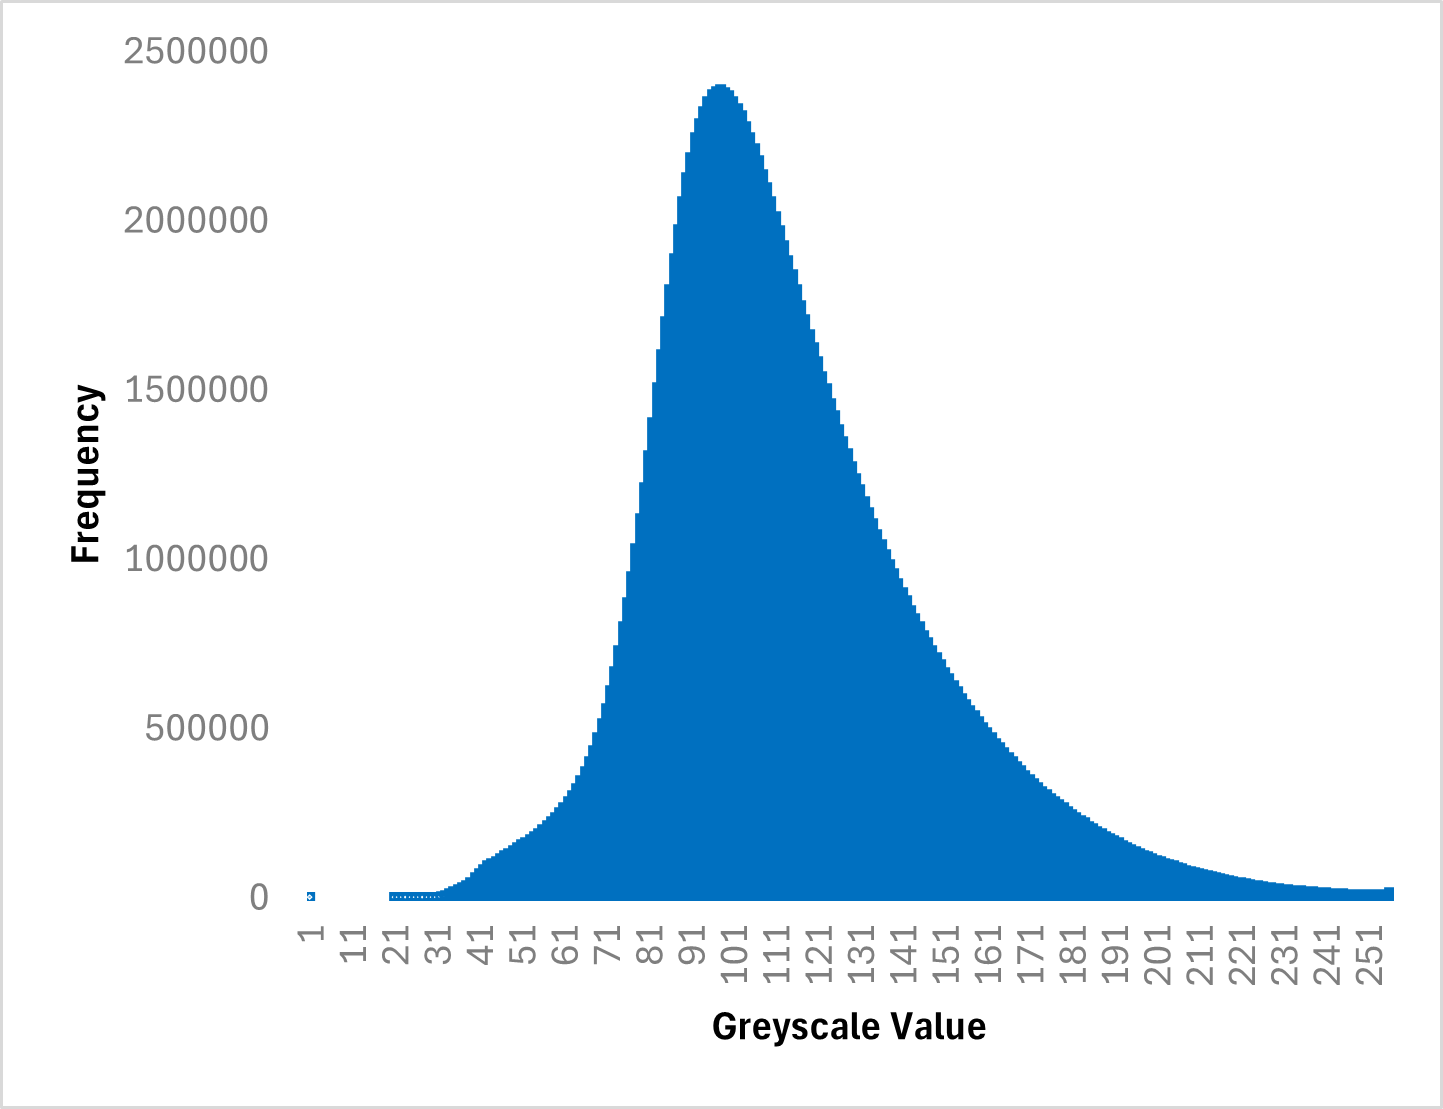
\includegraphics[width=0.45\textwidth]{./Media/IG430F Greyscale Histogram.png}
		\caption{PLACEHOLDER DRAFT: Histogram of greyscale values for IG-430 Sample F, 1000×, Showing skewness and unimodality}
		\label{fig:histogramnobimodal}
	\end{figure} 

	\begin{figure}[!htbp]
		\centering
		\includegraphics[width=0.45\textwidth]{./Media/MontageIG430C Methods.jpg}
		\caption{Thresholded Micrograph of IG-430 Sample C at $1000\times$ Magnification. Methods are labelled sequentially from right to left, row by row. (a) Default
			(b) Huang
			(c) Huang2
			(d) Intermodes
			(e) IsoData
			(f) Li
			(g) MaxEntropy
			(h) Mean
			(i) MinError(I)
			(j) Minimum
			(k) Moments
			(l) Otsu
			(m) Percentile
			(n) RenyiEntropy
			(o) Shanbhag
			(p) Triangle
			(q) Yen}
		\label{fig:Try All Thresholding Methods}
	\end{figure}  

	A HITL (human in the loop) approach was therefore undertaken, as illustrated
	in the  process diagram (Figure ~\ref{fig:Final Workflow}). Here, the operator
	subsamples the overall fused compsite, then examines this subsample to
	determine the threshold at which porosity and bulk are best separated. The
	operator then applies this threshold, along with a pore diameter threshold, to
	the full composite. The results are classified as either porosity or bulk to
	derive channel porosity.
	
\begin{figure}[!htbp]
    \centering
    \includegraphics[width=0.45\textwidth]{./Media/Newprocessmodel.png}
    \caption{Full thresholding workflow detailing the process of micrograph generation,
     composite assembly, subsampling, intensity thresholding, and pore diameter thresholding.}
    \label{fig:Final Workflow}
\end{figure}

	\subsubsection{Pore Diameter Thresholding}
    
  Pore size thresholds were imposed in this work, following previous studies
  \citep{Taylor2016, Huang2019, Kane2011a}, to restrict the automated
  recognition of pores to a range (i.e., only counting pores > 12.5µm\(^2\))
  where classification is deemed reliable. However, this approach is inherently
  limited by the practical difficulty of objectively determining whether any
  given pore classification is correct.
      
  As shown in (Table ~\ref{tab:thresholdsandvariationsIG430F}), extreme changes
  in the total pore count result from minor alterations in the threshold, with a
  0.5 µm\(^2\) threshold yielding a total pore count of 11,375, while a 1
  µm\(^2\) threshold yields a pore count of 6,485. Crucially however the total
  area of pores above the threshold remains relatively stable, with a porosity
  of 3.8\% for the 0.5 µm\(^2\) threshold, and 3.6\% for the 1 µm\(^2\)
  threshold. When combined with individual analyses of the resulting PSDs and
  precise examination of exactly which features are excluded at each
  threshold as per (Figure ~\ref{fig:improvedporediademo}), it is clear that a
  pore area threshold of 1 µm\(^2\) (dia = 1.12 µm) was the optimal compromise
  between type I and II errors.

   Crucially, setting such a threshold does not imply that no pores exist below
   this limit. Rather, it acknowledges that the confidence in classifying pores
   below the threshold is too low for reliable use. In this work, the
   limitations of any single technique are compensated by the strengths of
   others. Furing modelling, we select an interval over which the channel
   porosity determined from SEM imaging can reliably constrain the outputs of
   the inverse modelling process. Thus, no type II errors are introduced in the
   final model due to pore size thresholding, thanks to the combined use of
   alternative techniques and the ability to specify an interval within
   PoreXpert v.3.

   \begin{table}
  \centering
  \caption{Effect of different pore area thresholds on IG-430F, showing the resulting pore count, total area, average pore size, and percentage area.}
  \label{tab:thresholdsandvariationsIG430F}
  \resizebox{\columnwidth}{!}{%
    \begin{tabular}{l c c c c c c}
      \hline
      \textbf{Area Threshold} ($\mu$m$^2$) & 0 & 0.5 & 1 & 2 & 4 & 8 \\
      \hline
      Count & 254261 & 11375 & 6485 & 4085 & 2812 & 1881 \\
      TotalArea ($\mu$m$^2$) & 71219 & 56722 & 53361 & 50063.63 & 46518 & 41161\\
      Avg. Size ($\mu$m$^2$) & 0.28 & 4.987 & 8.229 & 12.255 & 16.543 & 21.883 \\
      \% Area & 4.786 & 3.812 & 3.586 & 3.364 & 3.126 & 2.766 \\
      \hline
    \end{tabular}%
  }
\end{table}

\begin{figure}[!htbp]
    \centering
    \includegraphics[width=0.35\textwidth]{./Media/ImprovedPoreDiaDemo.png}
    \caption{Effect of minimum area threshold on pore identification in subsample of IG-110 Sample B. Highlighted circles denote features which surpassed the previous threshold(s) only, indicated by colour. Thresholds applied (a–f, left-to-right, top-to-bottom): None, 0.5 µm\(^2\), 1 µm\(^2\), 2 µm\(^2\), 4 µm\(^2\), and 8 µm\(^2\).}
    \label{fig:improvedporediademo}
\end{figure}

\subsubsection{Channel Porosity Analysis and Calculation}
Following the determination of the above thresholds, the channel porosity was
calculated using the “Analyse Particles” function in ImageJ. This function scans
the micrograph pixel by pixel, identifies all pixels that surpass the intensity
threshold, and groups them into connected regions via a flood-fill algorithm.
Connectivity is defined based on the 8-connected (Moore neighborhood) criterion,
whereby a pixel at $(x,y)$ is considered connected to its eight immediate
neighbors:

\begin{multline*}
\footnotesize
(x-1,y-1),\; (x-1,y),\; (x-1,y+1),\; (x,y-1),\\[4pt]
(x,y+1),\; (x+1,y-1),\; (x+1,y),\; (x+1,y+1)
\end{multline*}


Thus, any two pixels that exceed the intensity threshold and are either directly
adjacent or diagonally connected are classified as belonging to the same region
(pore). The function then computes the area of each pore by converting the pixel
count into physical area (i.e., 10 pixels per micrometre). Regions that do not
meet the area threshold are omitted. The final results are a pore size
distribution (PSD) and the channel porosity (\%).


\subsection{Helium (He) Pycnometry}
	
Skeletal density was obtained using a Pycnomatic ATC pycnometer (Thermo Fisher
Scientific, Italy) at a temperature of 20.00 ± 0.01\textdegree{}C. Measurements
were taken in ten replicates per sample, calculating the arithmetic mean.

Solid phase volume $V_{\mathrm{SOLID}}$ was calculated assuming a theoretical
density of \todo{insert theoretical density here} g cm$^{-3}$ for an ideal
graphite crystal. Closed Pore Volume (CPV) and Open Pore Volume (OPV) for each
of the samples was calculated via equations \ref{eq:CPV} and \ref{eq:OPV}.

\begin{equation}
\mathrm{CPV} = \frac{m - V_{\mathrm{SOLID}} \times \rho{_\mathrm{s}}}{\rho{_\mathrm{s}}} 	\label{eq:CPV} 
\end{equation}

\begin{equation}
	\mathrm{OPV} = V_{\mathrm{BULK}} - \mathrm{CPV} - V_{\mathrm{SOLID}}\label{eq:OPV} 
\end{equation}

Specific Pore Volume (SPV), the void volume accessible to helium per gram of
sample was calculated via Equation \ref{eq:SPV}. 

\begin{equation}
\mathrm{SPV} = \frac{1}{\rho}-\frac{1}{\rho_\mathrm{s}}\label{eq:SPV} 
\end{equation}

\subsection{Mercury (Hg) Intrusion Porosimetry}
Mercury intrusion porosimetry operates on the fundamental principle that the
pressure at which a non-wetting fluid intrudes a given pore is inversely
proportional to the diameter of that pore (i.e., the larger the pore, the easier
it is for the non-wetting fluid to enter it). The exact physical relationship
between diameter and applied pressure is governed by the Laplace Equation (Eq.
~\ref{eq:washburn})
	
	\begin{equation} \label{eq:washburn}
		d = \frac{-4\gamma \cos \theta}{P}
	\end{equation}

		The pore diameter \(d\) is calculated using the equation:
	\begin{itemize}
		\item $d$ (m): Pore diameter
		\item $\gamma$ (N/m): Surface tension of the fluid
		\item $\theta$ (degrees): Contact angle of the fluid with the surface
		\item $Papp$ (P): Pressure
	\end{itemize}

Values of 140$^{\circ}$ and 130$^{\circ}$ were used for advancing and receding
contact angles respectively, while a value of 0.480 N m$^{-1}$ was assumed for the
surface tension of mercury \citep{VANBRAKEL19811}. 

In this work, the dataset generated by Jones et al. \citep{Jones2018} was used,
representing measurements performed not only on the same grades of graphite, but
the same batch of graphites (i.e. sampled from the same larger "brick") as those samples
which underwent SEM imaging and He pycnometry in this work.

\subsection{Nitrogen (N$_2$) Adsorption}
Low-pressure gas adsorption isotherms were obtained using a BELSORP-max
volumetric gas adsorption instrument (MicrotracBEL, Japan). 


As with mercury intrusion porosimetry, the dataset generated by Jones et al.
\citep{Jones2018} was used in this work. Once more, this represents
measurements performed on the same grades but the same
batch of graphites (i.e. sampled from the same larger "brick") as those samples which
underwent SEM imaging and He pycnometry in this work.

\section{{Modelling}}
Hg intrusion porosimetry cannot capture the full range of pore sizes
 Hence, the use of GCMC to "stitch" together the pore diameter
ranges covered by both Hg and He adsorption \citep{Jones2018}. The pore size distribution (PSD) is
generated by combining the methods into a single set of values, which PoreXpert
inversely models to capture. 

\clearpage

\bibliography{bibliography}
\end{document}